\documentclass[11pt,a4paper]{article}

% --- Codificación e idioma ---
\usepackage[utf8]{inputenc}
\usepackage[T1]{fontenc}
\usepackage[spanish, es-tabla]{babel}

% --- Paquetes matemáticos ---
\usepackage{amsmath}
\usepackage{amssymb}

% --- Tipografía: Times New Roman---
\usepackage{mathptmx}

% --- Márgenes: 2.5 cm en todos los lados---
\usepackage[a4paper, margin=2.5cm]{geometry}

% --- Interlineado: 1.5 líneas---
\usepackage{setspace}
\onehalfspacing

% --- Formato de títulos y subtítulos---
\usepackage{titlesec}
\titleformat{\section}
  {\fontsize{16}{20}\selectfont\bfseries}
  {\thesection}{1em}{}
\titleformat{\subsection}
  {\fontsize{14}{18}\selectfont\bfseries}
  {\thesubsection}{1em}{}
\titleformat{\subsubsection}
  {\fontsize{12}{15}\selectfont\bfseries}
  {\thesubsubsection}{1em}{}

% --- Carátula UBA (DC/Exactas) ---
\usepackage[sinEntregas]{caratula}

% --- Figuras: se compila desde la carpeta informe/ y las figuras están en resultados/figuras/ ---
\graphicspath{{../resultados/figuras/}}

% --- Tablas profesionales ---
\usepackage{booktabs}
\usepackage{array}
\usepackage{caption}
\captionsetup{font=small, labelfont=bf, skip=8pt}

% --- Hipervínculos ---
\usepackage{hyperref}
\hypersetup{
    colorlinks=true,
    linkcolor=black,
    citecolor=blue,
    urlcolor=blue
}

\begin{document}

% ==============================================================================
% 1. CARÁTULA
% ==============================================================================
\pagenumbering{gobble} % Sin número de página en la carátula

\titulo{Análisis Microclimático y Riesgo Biológico en Salas de Colecciones del MACN}
\subtitulo{Modelado del efecto climático exterior sobre la temperatura interna y la proliferación de plagas}

\fecha{\today}
\materia{Casos de Estudio en Estadística}
\submateria{Solicitante: Soledad Tancoff (MACN)}
\grupo{Grupo 3}

% Integrantes del grupo (Nombre, LU, email)
\integrante{Calo, Agustín}{390/23}{caloagustin4@ejemplo.com}
\integrante{Cogno, Matías}{944/22}{matysbn@gmail.com}
\integrante{Bravo, Ivan Agustín}{786/23}{bravoivanagustin@gmail.com}
\integrante{Kiss, Delfina}{72/23}{kissdelfina@gmail.com}


\maketitle

\newpage
\pagenumbering{arabic} % Numeración arábiga desde el Resumen

% ==============================================================================
% 2. RESUMEN (Aproximadamente 1 página según pautas)
% ==============================================================================
\section{Resumen}

\textbf{Contexto y Problema:} La conservación preventiva de colecciones de material orgánico históricas depende críticamente de la estabilidad microclimática en las salas de guarda. Variaciones bruscas de temperatura o niveles elevados de humedad relativa pueden provocar fatiga estructural en los ejemplares o favorecer la proliferación de insectos perjudiciales como los son los coleópteros y lepidópteros. En este trabajo se analiza el grado de acoplamiento térmico entre las condiciones meteorológicas exteriores registradas por el Servicio Meteorológico Nacional (SMN) y el microclima interno de diversas salas del Museo Argentino de Ciencias Naturales (MACN) y colecciones asociadas, evaluando asimismo la relación con las capturas de insectos en trampas de monitoreo.

\textbf{Metodología:} Se procesaron registros continuos de temperatura y humedad capturados por un conjunto reducido de sensores HOBO. Estos fueron colocados, generalmente a lo largo de todo un año, en alguno de los catorce sectores o salas del museo, exceptuando ciertas ocaciones donde se ubicaron dos en la misma sala con fines particulares. Para evitar inferencias espurias debidas a la fuerte autocorrelación temporal, se ajustaron modelos de mínimos cuadrados generalizados (GLS) con estructura autorregresiva de primer orden ($AR(1)$) y armónicos anuales. La inercia térmica de cada espacio se determinó mediante la comparación de ventanas de promedio móvil exterior. Paralelamente, se exploraron las tasas de captura de insectos mediante modelos para datos de conteo con offset temporal para estandarizar los intervalos de exposición.

\textbf{Principales Hallazgos:} Los resultados revelan dos regímenes térmicos bien diferenciados dentro del museo: (1) \textit{Salas permeables o expuestas} (e.g., Paleovertebrados Anexo y Arácnidos), caracterizadas por una rápida respuesta al exterior (inercia de 2 días), pendientes elevadas ($\beta \approx 0{,}50 - 0{,}62\,^\circ\text{C}_\text{int}/^\circ\text{C}_\text{ext}$) y una marcada amplitud térmica diaria; y (2) \textit{Salas aisladas o con alta inercia} (e.g., Ictiología Colección, Ornitología y Paleovertebrados Ameghino), que presentan una inercia de 4 a 7 días, menor transmisión de calor ($\beta \approx 0{,}07 - 0{,}17$) y una memoria propia dominante ($\phi > 0{,}90$). En cuanto al riesgo biológico, la tasa diaria de capturas de plagas exhibe una fuerte estacionalidad asociada a la temperatura ($p = 0{,}017$), observándose un incremento de la actividad en los meses estivales.

\textbf{Implicancias:} Los hallazgos permiten identificar qué sectores requieren intervención prioritaria en aislamiento pasivo o acondicionamiento climático activo, y justifican el establecimiento de calendarios de monitoreo y control de plagas intensificados al comienzo de la temporada estival.

\newpage

% ==============================================================================
% 3. INTRODUCCIÓN Y OBJETIVOS
% ==============================================================================
\section{Introducción y Objetivos}

Las colecciones de historia natural albergan bienes culturales y científicos irremplazables cuya preservación a largo plazo está condicionada por el ambiente de guarda...

\subsection{Preguntas de investigación e hipótesis}
\begin{enumerate}
    \item ¿En qué medida y con qué retardo temporal penetran las fluctuaciones meteorológicas exteriores en las salas del museo?
    \item ¿Presentan todas las salas el mismo nivel de aislamiento o existen diferencias edilicias sustanciales?
    \item ¿Se observa una correlación entre el microclima y la proliferación de insectos plaga en las colecciones?
\end{enumerate}

% ==============================================================================
% 4. METODOLOGÍA
% ==============================================================================
\section{Metodología}

\subsection{Fuente de datos}
Se utilizaron dos fuentes de datos principales, siendo estas mediciones de las condiciones internas mediante sensores y registros históricos de clima en la Ciudad de Buenos Aires provisto por el Servicio Meteorológico Nacional.
Los datos de interiores fueron captados por dispositivos \href{https://www.hobodataloggers.com/products/data-loggers/mx2301a?zCountry=AR}{HOBO}, capaces de tomar medidas de la temperatura y humedad relativa del ambiente en intervalos fijos de tiempo con un error aproximado de un minuto. La temperatura medida tiene un error ±0.2°C en el rango de 0 hasta 70°C y la humedad de ±2.5\% entre 10\% y 90\%. Su resolución de temperatura es de 0.02-0.04°C con un corrimiento anual menor a 0.01°C y para humedad es de 0.01\% con corrimiento menor a 1\% anual. Los intervalos de tiempo presentenes en nuestros datos son variables, siendo el preponderante el de cada cuatro horas.
Estos fueron colocados en alguna de las 14 secciones etiquetas, que pueden ser la sala entera o una región de la misma. El tiempo que se encuentran en determinada ubicación depende de si se encuentran allí para monitorear situaciones puntuales o como control general. Por esta razón cada sala cuenta con una cantidad variable de mediciones a lo largo de uno o varios años como podemos observar en la Tabla~\ref{tab:años_por_sala}, por lo cual la evidencia para cada modelo varía según la sala.

\begin{table}[ht]
\centering
\begin{tabular}{llr @{\hspace{2em}} llr}
\toprule
\textbf{Serie} & \textbf{Años} & \textbf{Días} & \textbf{Serie} & \textbf{Años} & \textbf{Días} \\
\midrule
BA-v              & 2014--2020  & 1269 & BA-Pb          & 2022--2023  & 325 \\
MACN-Ict Colección  & 2022--2025  & 710  & MACN-Pv General  & 2019        & 303 \\
MACN-Or Antigua   & 2020--2021  & 693  & MACN-Pv Ameghino & 2019        & 269 \\
MACN-Ict Laboratorio & 2022--2023 & 398  & MACN-He        & 2014 y 2016 & 194 \\
MACN-Pv Anexo     & 2019--2020  & 366  & MACN-Ar        & 2016        & 78  \\
MACN-Or Azara     & 2021        & 357  & MACN-In Arriba & 2025        & 52  \\
MACN-Ma           & 2016 y 2020 & 332  & MACN-In Abajo  & 2025        & 52  \\
\bottomrule
\end{tabular}
\caption{Años y cantidad de días con mediciones por sala.}
\label{tab:años_por_sala}
\end{table}

Por otro lado, los datos del exterior fueron extraídos de los \href{https://www.smn.gob.ar/descarga-de-datos}{datos abiertos} del Servicio Meteorológico Nacional, estructurados en dos csv con datos del clima diario de cada estación meteorológica del país desde 1991 hasta el 2026. De estas mediciones tomamos aquellas pertenecientes al Observatorio Central de Buenos Aires (OCBA) que son a nivel de día, donde está presente el registro de la temperatura máxima, media, mínima y humedad relativa entre otros. 

Finalmente, contamos con registros de capturas de coleópteros y lepidópteros en las salas MACN-Ba, MACN-En y MACN-Ma entre 2019 y 2020. Las trampas utilizadas, tanto aereas como terrestres, están basadas en feromonas. La cantidad de insectos atrapados fue anotada cada dos semanas con un cese en el periodo invernal (aproximadamente de julio a octubre/noviembre) debido a una menor aparición de los mismos.

\subsection{Procesamiento y limpieza de datos}
Para tener un registro completo y estandarizado, se eliminaron las observaciones de los bordes, es decir, el primer y último día de muestreo de cada despliegue por estar incompletos. Asimismo, se corrigió la identificación de dataloggers superpuestos en series complejas como Ornitología (diferenciando las colecciones Antigua y Azara)...

\subsection{Estrategia de modelado estadístico}
\subsubsection{Caso de la temperatura}
Se decidió tomar como variables a predecir la temperatura máxima y mínima de la sala, elegida como el máximo y el mínimo respectivamente entre las observadas por tener una correspondencia directa con las mismas presentes en los datos del SMN. Para inferir ($T_{\text{max, int}}$) y ($T_{\text{min, int}}$) primero se implementaron modelos de regresión lineal generalizada de la siguiente forma:
\begin{equation}
    T_{\text{max, int}}(t) = \beta_0 + \beta_1 \, \overline{T}_{\text{max, ext } k}(t) + \gamma_1 \sin\left(\frac{2\pi t}{365{,}25}\right) + \gamma_2 \cos\left(\frac{2\pi t}{365{,}25}\right) + \varepsilon(t) 
    \\
\end{equation}
\begin{equation}
    T_{\text{min, int}}(t) = \beta_0 + \beta_1 \, \overline{T}_{\text{min, ext } k}(t) + \gamma_1 \sin\left(\frac{2\pi t}{365{,}25}\right) + \gamma_2 \cos\left(\frac{2\pi t}{365{,}25}\right) + \varepsilon(t)
\end{equation}
En estas ecuaciones $\overline{T}_{\text{ext, } k}$ y  representan el promedio móvil exterior de $k$ días y $\varepsilon(t) = \phi \, \varepsilon(t-1) + u(t)$ captura la fuerte autocorrelación serial intrínseca de los datos diarios ($AR(1)$). Este intenta resumir la información de temperatura durante el mísmo día y los $k-1$ previos al que se busca predecir. La importancia de tener información pasada es por el efecto aislante que puede tener la infraestructura del museo, es decir, los materiales de muros, ventanas y puertas sumado a condiciones propias de los ambientes pueden hacer que los efectos climáticos lleguen con retraso. Asimismo, las funciones sinusoidales del tiempo buscan representar el efecto de la estación, pues mapean los 365.25 días del año al intervalo $[-1,1]$ lo cual permite conectar el día 1 con el 365.

Posteriormente se implementó un modelo rezagado, generalmente usado en series de tiempo, conocido como modelo de rezagos distribuidos que no solo contiene la correlación de los errores por ser días consecutivos si no también incorpora como variables predictoras a los k-1 días previos al evento como se ve en las ecuaciones~\ref{eq:ecuacion_rezagados_max} y ~\ref{eq:ecuacion_rezagados_min}.

\begin{equation}
T_{\text{max, int}}(t) = \beta_0 + \, \sum_{i=t-k}^{t}\beta_iT_{\text{max, ext, } i} + \gamma_1 \sin\left(\frac{2\pi t}{365{,}25}\right) + \gamma_2 \cos\left(\frac{2\pi t}{365{,}25}\right) + \varepsilon(t)
\label{eq:ecuacion_rezagados_max}
\end{equation}
\\
\begin{equation}
T_{\text{min, int}}(t) = \beta_0 + \, \sum_{i=t-k}^{t}\beta_iT_{\text{min, ext, } i} + \gamma_1 \sin\left(\frac{2\pi t}{365{,}25}\right) + \gamma_2 \cos\left(\frac{2\pi t}{365{,}25}\right) + \varepsilon(t)
\label{eq:ecuacion_rezagados_min}
\end{equation}

Se puede apreciar como el modelo de promedio es un caso particular de este, donde los coeficientes de los días son iguales y se encuentran divididos por k, por lo que este modelo a pesar de tener más complejidad tiene mayor capacidad expresiva. Se experimentó con k para encontrar la cantidad de días necesarios para tener la mejor explicación de la temperatura interna en cada una de las salas.

Por último, se tomaron las ecuaciones~\ref{eq:ecuacion_rezagados_max} y ~\ref{eq:ecuacion_rezagados_min} y se suprimió el uso de la variable predictora que corresponde al mismo día $t$. Esta decisión se tomo con dos objetivos: primero, observar que tan importante es el efecto directo de la temperatura exterior y, segundo, ver que la factibilidad de predecir la temperatura interior el día $t$ a partir de la exterior en los $k-1$ días anteriores. La evaluación llevada a cabo fue por una ventana deslizante, es decir, se entrena al modelo con $p$ días y se ve que tan bien predice el día $p+1$, consiguiendo una evaluación de desempeño moviendo el p por una unidad. 

\subsubsection{Caso de predicción de plagas}
Para estudiar la aparición de coleópteros y lepidópteros propusimos un modelo lineal generalizado poisson. Esta elección es sirve como base para cualquier problema de conteo (es decir, predicción de un número entero positivo de eventos en el tiempo) y usamos una ecuación de la forma:

\begin{equation}
Y \sim Poisson(\lambda) \\
\end{equation}
\begin{equation}
log(\mathbb{E}[Y]) = \beta_0 + \beta_1 Temp + \beta_2 Hum +\epsilon_t
\label{eq:modelo_poisson}
\end{equation}

% ==============================================================================
% 5. RESULTADOS
% ==============================================================================
\section{Resultados}

\subsection{Sensibilidad térmica e inercia por sala}
En la Tabla~\ref{tab:inercia} se resumen los parámetros estimados para cada una de las salas analizadas.

\begin{table}[htbp]
\centering
\small
\caption{Resultados del modelo GLS con estructura $AR(1)$ para cada sala y subsector.}
\label{tab:inercia}
\begin{tabular}{l c c c c c}
\toprule
\textbf{Sala / Subsector} & \textbf{N (días)} & \textbf{Inercia óptima} & \textbf{Pendiente $\beta$ ($\pm$ EE)} & \textbf{$\phi$ (AR1)} & \textbf{$R^2$} \\
\midrule
MACN\_Ar - General     & 76   & 2 días & 0,617 (0,103) & 0,557 & 0,829 \\
MACN\_Pv - Anexo       & 364  & 2 días & 0,540 (0,028) & 0,480 & 0,946 \\
BA\_v - General        & 1267 & 2 días & 0,397 (0,010) & 0,830 & 0,966 \\
MACN\_Ict - Laboratorio& 396  & 3 días & 0,222 (0,012) & 0,872 & 0,977 \\
MACN\_Ma - General     & 330  & 3 días & 0,194 (0,012) & 0,933 & 0,970 \\
MACN\_Pv - Ameghino    & 267  & 4 días & 0,124 (0,013) & 0,905 & 0,945 \\
MACN\_Ict - Colección  & 708  & 7 días & 0,105 (0,009) & 0,963 & 0,950 \\
MACN\_Or - Azara       & 355  & 7 días & 0,091 (0,011) & 0,937 & 0,964 \\
MACN\_Or - Antigua     & 691  & 7 días & 0,073 (0,007) & 0,958 & 0,959 \\
\bottomrule
\end{tabular}
\end{table}

La Figura~\ref{fig:modelo_pv} ilustra el contraste de comportamiento térmico en Paleovertebrados: mientras el subsector Anexo copia fuertemente las ondas de calor y frío del exterior, el subsector Ameghino exhibe una marcada amortiguación e inercia térmica.

\begin{figure}[htbp]
  \centering
  % Al especificar únicamente el ancho (width), LaTeX preserva automáticamente la proporción original
  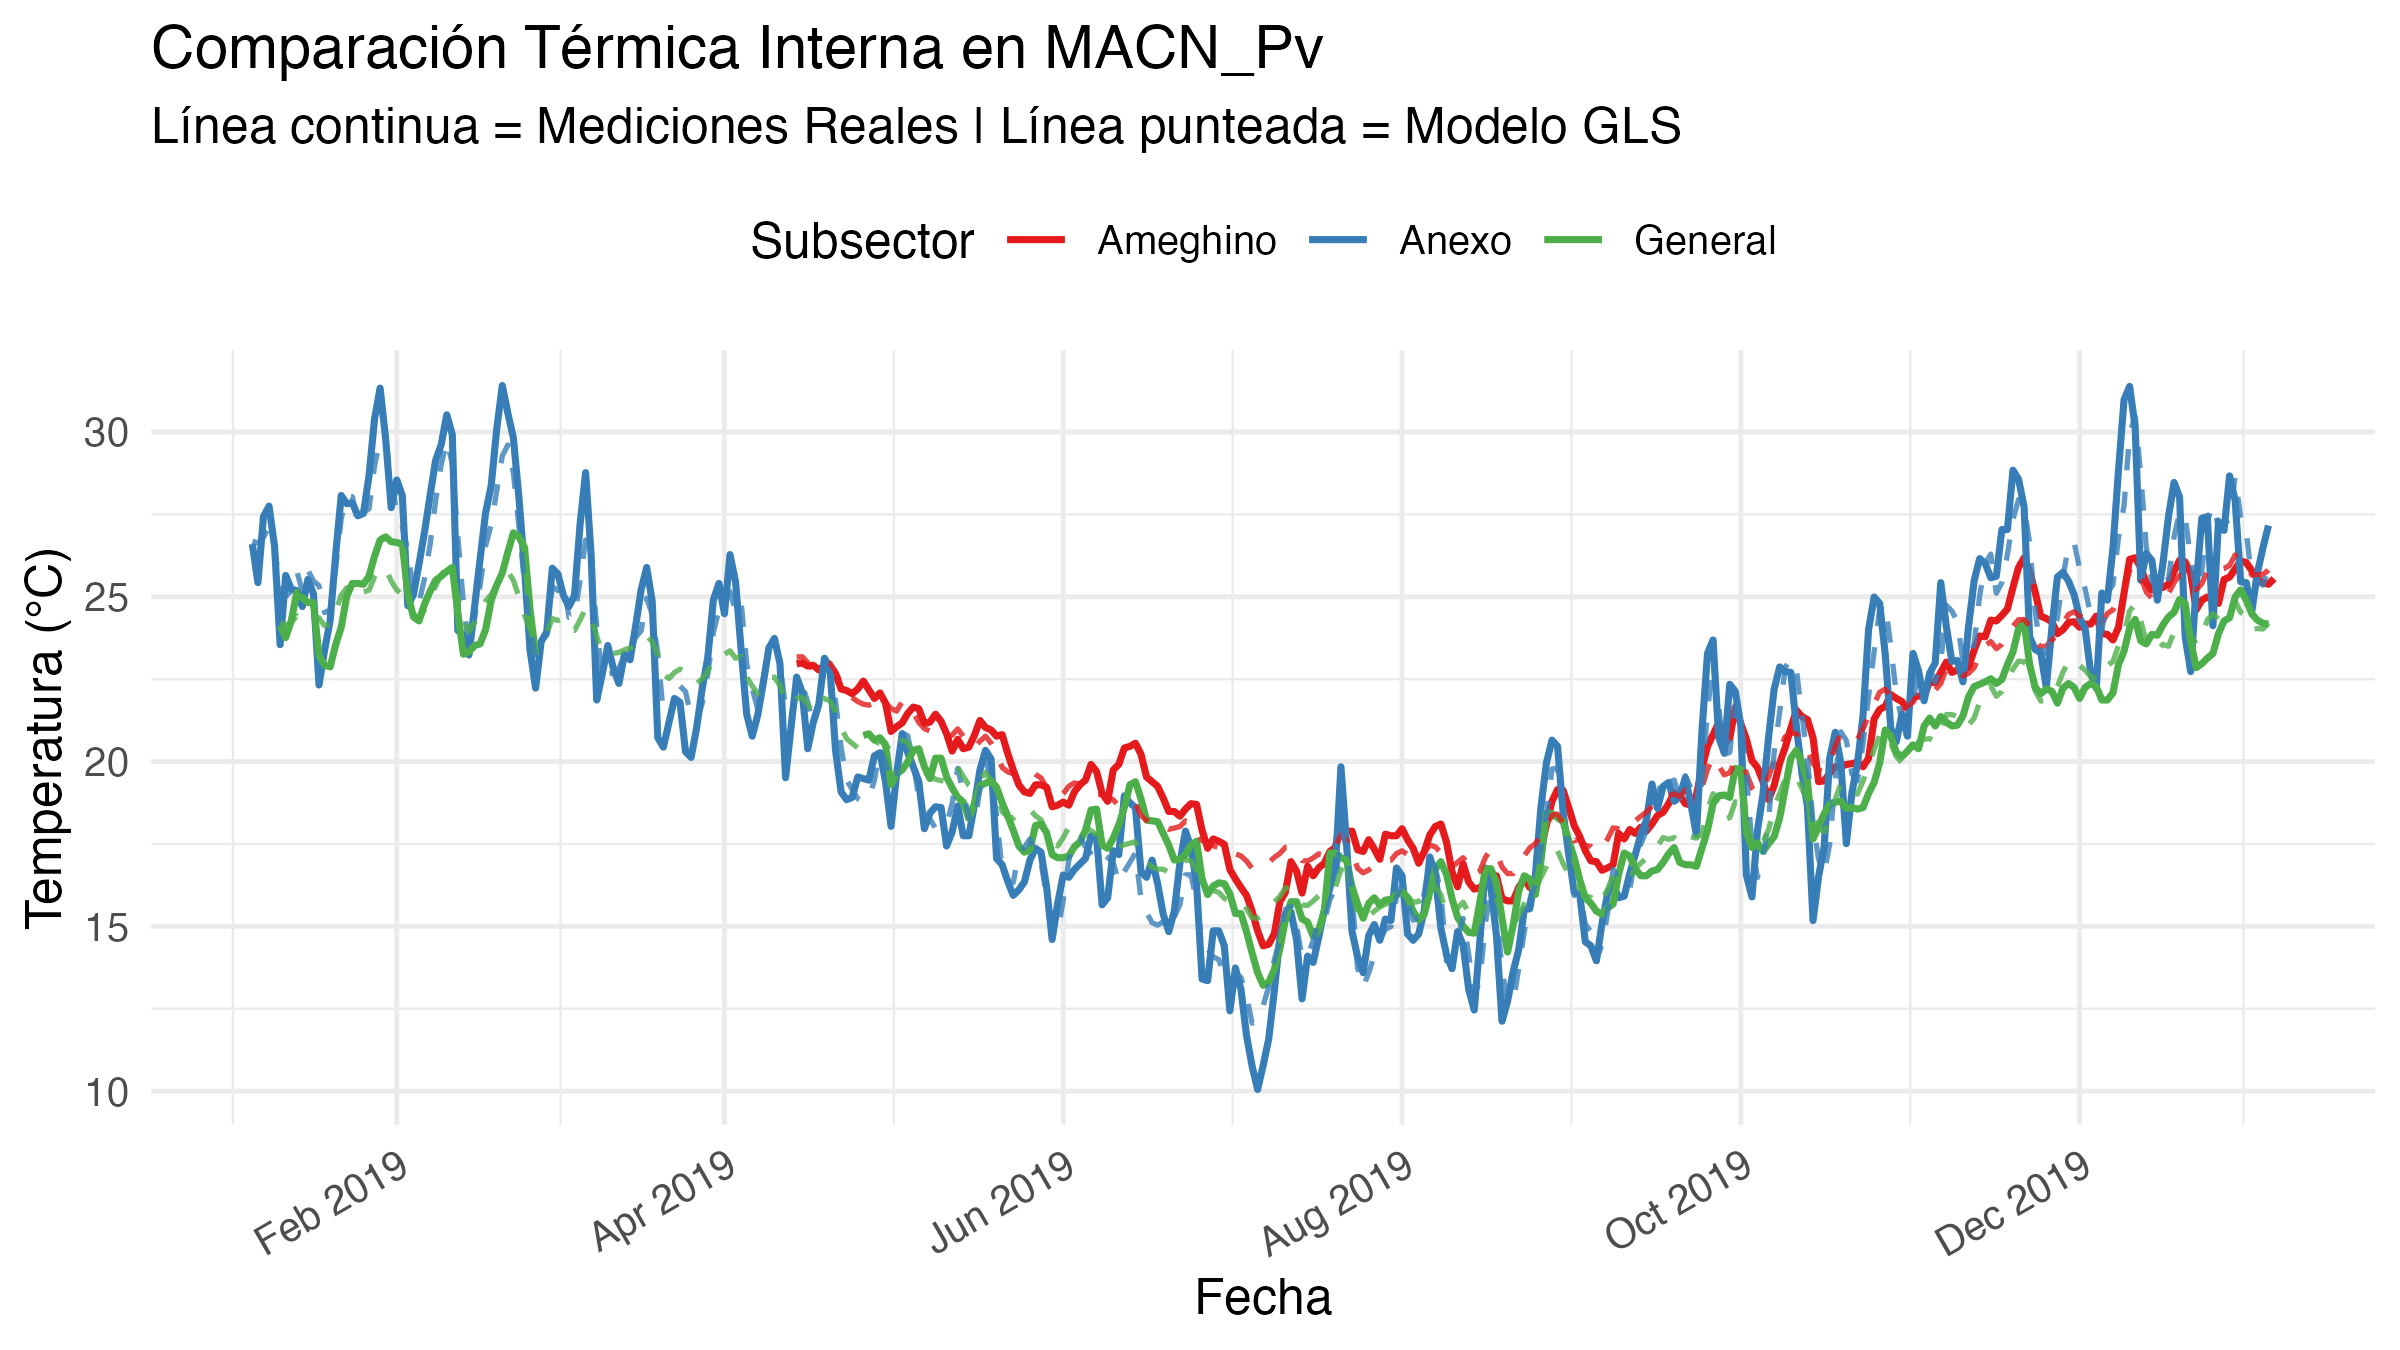
\includegraphics[width=0.88\textwidth]{fig_modelo_pv.png}
  \caption{Ajuste del modelo GLS en Paleovertebrados (MACN\_Pv). Línea continua: mediciones observadas; línea punteada: predicción del modelo GLS.}
  \label{fig:modelo_pv}
\end{figure}

\subsection{Dinámica de insectos plaga y condiciones ambientales}
El análisis exploratorio de las trampas de coleópteros y lepidópteros indica una clara correspondencia entre las temperaturas estivales y el incremento en las tasas de captura (Figura~\ref{fig:trampas_temp}).

\begin{figure}[htbp]
  \centering
  % Ancho ajustado proporcionalmente sin deformación
  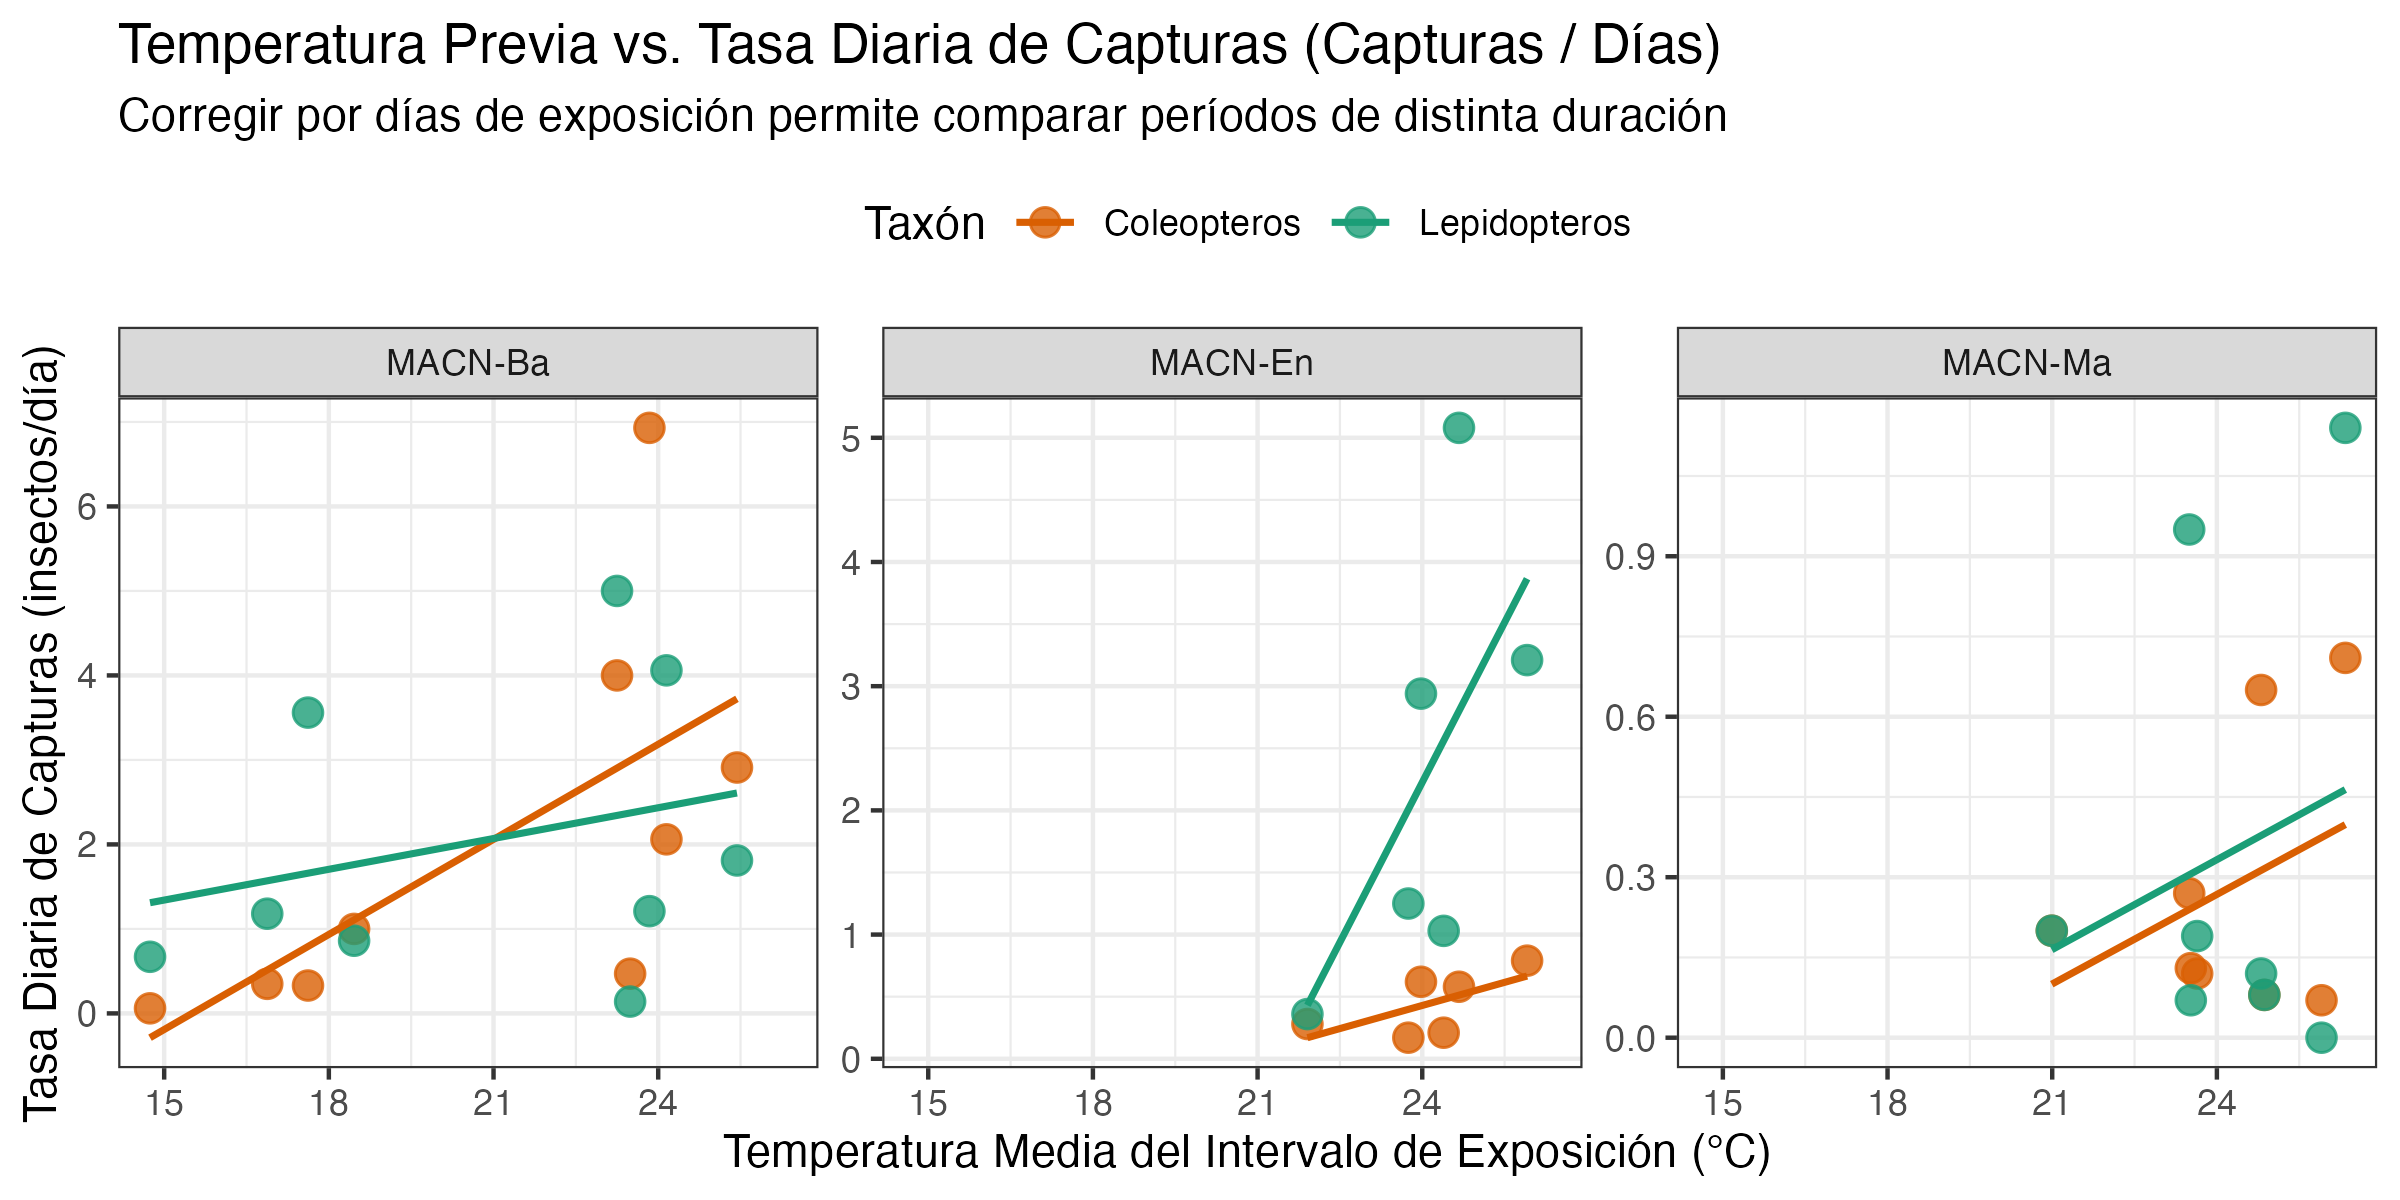
\includegraphics[width=0.88\textwidth]{fig_trampas_temperatura.png}
  \caption{Relación entre la temperatura previa y la tasa diaria de capturas por sala y taxón. La normalización por días de exposición permite comparar períodos de diferente duración.}
  \label{fig:trampas_temp}
\end{figure}

% ==============================================================================
% 6. DISCUSIÓN Y CONCLUSIONES
% ==============================================================================
\section{Discusión y Conclusiones}

\subsection{Interpretación disciplinar y recomendaciones}
Se identifican dos tipologías edilicias en el museo: salas expuestas que requieren refuerzo de aislamiento térmico, y salas protegidas que mantienen una elevada estabilidad pasiva...

\subsection{Limitaciones del estudio}
Es necesario señalar que el muestreo de trampas biológicas presentó revisiones muy espaciadas e intervalos desiguales (desde 9 hasta 161 días), lo cual restringe la posibilidad de predecir capturas en horizontes de corto plazo. No obstante, el control por tiempo de exposición mediante modelos con offset permite extraer conclusiones válidas sobre la estacionalidad del riesgo...

% ==============================================================================
% 7. REFERENCIAS BIBLIOGRÁFICAS
% ==============================================================================
\section{Referencias}
\begin{itemize}
    \item Pinheiro, J. C., \& Bates, D. M. (2000). \textit{Mixed-effects models in S and S-PLUS}. Springer.
    \item R Core Team (2023). \textit{R: A language and environment for statistical computing}. R Foundation for Statistical Computing, Vienna, Austria.
    \item Thomson, G. (1986). \textit{The Museum Environment}. Butterworth-Heinemann.
\end{itemize}

% ==============================================================================
% 8. ANEXOS (Opcional, máximo 5 carillas)
% ==============================================================================
\appendix
\section{Anexos}
Diagnósticos complementarios de residuos y tablas auxiliares...

\end{document}
